\documentclass{sigchi}

% Use this command to override the default ACM copyright statement (e.g. for preprints). 
% Consult the conference website for the camera-ready copyright statement.


%% EXAMPLE BEGIN -- HOW TO OVERRIDE THE DEFAULT COPYRIGHT STRIP -- (July 22, 2013 - Paul Baumann)
% \toappear{Permission to make digital or hard copies of all or part of this work for personal or classroom use is 	granted without fee provided that copies are not made or distributed for profit or commercial advantage and that copies bear this notice and the full citation on the first page. Copyrights for components of this work owned by others than ACM must be honored. Abstracting with credit is permitted. To copy otherwise, or republish, to post on servers or to redistribute to lists, requires prior specific permission and/or a fee. Request permissions from permissions@acm.org. \\
% {\emph{CHI'14}}, April 26--May 1, 2014, Toronto, Canada. \\
% Copyright \copyright~2014 ACM ISBN/14/04...\$15.00. \\
% DOI string from ACM form confirmation}
%% EXAMPLE END -- HOW TO OVERRIDE THE DEFAULT COPYRIGHT STRIP -- (July 22, 2013 - Paul Baumann)


% Arabic page numbers for submission. 
% Remove this line to eliminate page numbers for the camera ready copy
\pagenumbering{arabic}


% Load basic packages
\usepackage{balance}  % to better equalize the last page
\usepackage{graphics} % for EPS, load graphicx instead
\usepackage{times}    % comment if you want LaTeX's default font
\usepackage{url}      % llt: nicely formatted URLs
% llt: Define a global style for URLs, rather that the default one
\makeatletter
\def\url@leostyle{%
  \@ifundefined{selectfont}{\def\UrlFont{\sf}}{\def\UrlFont{\small\bf\ttfamily}}}
\makeatother
\urlstyle{leo}

\usepackage{gensymb}
\usepackage{afterpage}
% see http://tex.stackexchange.com/questions/46055/typesetting-with-inch-symbols-and-sizes-in-inches
% \usepackage{mathpazo}
\usepackage{amsmath}
\def\inch#1{#1''}
\def\ft#1{#1'\thinspace}



% comment macros are in inputmacros.tex
% set up tight list spacing
\usepackage{enumitem} 
\setlist{nolistsep,nosep}

% for toggles
\usepackage{etoolbox}

\newcommand {\studyquote}[1]{\em ``#1''\normalfont}

% CHANGE FROM TOGGLE TRUE TO TOGGLE FALSE FOR NON-ANONYMOUS RENDERING
% http://tex.stackexchange.com/questions/5894/latex-conditional-expression
\newtoggle{anonymous}
%\togglefalse{anonymous}
\toggletrue{anonymous}

% CHANGE FROM TOGGLE TRUE TO TOGGLE FALSE TO HIDE COMMENTS
\newtoggle{comments}
%\toggletrue{comments}
\togglefalse{comments}

% Comment region command (from Wesley Willett)
\usepackage[usenames]{color}
\usepackage[usenames,dvipsnames]{xcolor}
\iftoggle{comments} {
  %if we want to show comments
  \newcommand {\claire}[1]{{\color{Orange}\bf{CT: #1}\normalfont}}
  \newcommand {\sean}[1]{{\color{BlueGreen}\bf{SC: #1}\normalfont}}
  \newcommand {\yang}[1]{{\color{NavyBlue}\bf{YL: #1}\normalfont}}
  \newcommand {\ben}[1]{{\color{violet}\bf{BZ: #1}\normalfont}}
  \newcommand {\bjoern}[1]{{\color{BrickRed}\bf{BH: #1}\normalfont}}
  \newcommand {\achal}[1]{{\color{OliveGreen}\bf{AD: #1}\normalfont}} % can't find another color...
  \newcommand {\changes}[1]{{\color{Red}\bf{#1}\normalfont}}
}{
  %if we don't want to show comments
  \newcommand {\claire}[1]{}
  \newcommand {\sean}[1]{}
  \newcommand {\yang}[1]{}
  \newcommand {\ben}[1]{}
  \newcommand {\bjoern}[1]{}
  \newcommand {\achal}[1]{}
  \newcommand {\changes}[1]{{#1}}
}
\newcommand {\systemname}{HOBS }
\newcommand {\systemnamenospace}{HOBS}

% To make various LaTeX processors do the right thing with page size.
\def\pprw{8.5in}
\def\pprh{11in}
\special{papersize=\pprw,\pprh}
\setlength{\paperwidth}{\pprw}
\setlength{\paperheight}{\pprh}
\setlength{\pdfpagewidth}{\pprw}
\setlength{\pdfpageheight}{\pprh}

% Make sure hyperref comes last of your loaded packages, 
% to give it a fighting chance of not being over-written, 
% since its job is to redefine many LaTeX commands.
\usepackage[pdftex]{hyperref}
\hypersetup{
pdftitle={SIGCHI Conference Proceedings Format},
pdfauthor={LaTeX},
pdfkeywords={SIGCHI, proceedings, archival format},
bookmarksnumbered,
pdfstartview={FitH},
colorlinks,
citecolor=black,
filecolor=black,
linkcolor=black,
urlcolor=black,
breaklinks=true,
}

% create a shortcut to typeset table headings
\newcommand\tabhead[1]{\small\textbf{#1}}


% End of preamble. Here it comes the document.
\begin{document}


% as we discussed last time, the "Sees" and "Line-of-sight" suggests some computer vision direction 
% need a different title for sure, but not in a hurry
\title{Head orientation-based target selection in physical spaces}
%Project GlasSees: Direct Interaction Through Line-of-sight}

\iftoggle{anonymous}{
\author{
 \alignauthor Anonymous for submission\\
    \affaddr{...}\\
    \email{...}\\
  }
}{ %else
  \numberofauthors{1}
  \author{
  \alignauthor Yu-Hsiang Chen$^{\dagger}$, Ben Zhang$^{\dagger}$, Claire Tuna$^{\dagger}$, Yang Li$^{\ddagger}$, Edward Lee$^{\dagger}$, Bj\"orn Hartmann$^{\dagger}$ \\
  \affaddr{$\dagger$: UC Berkeley EECS \& CITRIS Invention Lab \hspace{0.25in} $\ddagger$: Google Research}\\
  \email{sean.yhc@gmail.com, benzh@eecs.berkeley.edu, clairetuna@gmail.com, yangli@acm.org, eal@eecs.berkeley.edu, bjoern@eecs.berkeley.edu}
  }
}

\maketitle

\begin{abstract}
%!TEX root = uist14.tex

%% Yang suggests: Interacting with smart objects in the physical space efficiently is a realistic challenge as these objects become ubiquitous. In this paper, we contribute HOBS, a set of novel methods for selecting physical objects at a distance using infrared-sensed head orientations. We augment a commercial head-worn device, Google Glass, with an infrared (IR) emitter to select targets equipped with IR receivers. We present the iterative design process of our methods, involving a series of interaction technique and hardware design and user evaluations....
Emerging head-worn computing devices can enable interactions with smart objects in physical spaces.
%
We present the iterative design and evaluation of \systemname -- a Head-Orientation Based Selection technique for interacting with these devices at a distance. We augment a commercial wearable device, Google Glass, with an infrared (IR) emitter to select targets equipped with IR receivers. Our first design shows that a naive IR implementation can outperform list selection, but has poor performance when refinement between multiple targets is needed. A second design uses IR intensity measurement at targets to improve refinement. To address the lack of natural mapping of on-screen target lists to spatial target location, our third design infers a spatial data structure of the targets enabling a natural head-motion based disambiguation.
%
Finally, we demonstrate a universal remote control application using HOBS and report qualitative user impressions.

\end{abstract}

\keywords{
  Wearable computing; tangible; smart devices; remote control; glass; infared
}

%% refer to http://www.acm.org/about/class/ccs98-html
\category{H.5.2.}{Information Interfaces and Presentation (e.g. HCI)}{Interaction styles (e.g., commands, menus, forms, direct manipulation)}.

\vfill\eject

%!TEX root = sui14.tex
\vfill
\section{Introduction}
%\bjoern{We should see if we can change language in a few places to strengthen the connection to ``Spatial User Interaction", the title of the conference.}

%% from the swarm vision to the necessity of selection
The number of smart objects in our environment with embedded computation and communication has grown rapidly. These objects are all potential targets for interaction. To initiate {\em spatial interactions}, a user needs to first acquire the target object -- a fundamental task that has been extensively studied in graphical user interfaces, but not yet well-explored in {\em physical spaces}.

\changes{Today, companies like Samsung and Whirlpool are making smart appliances with companion applications that use smartphones as {\em universal remote controls}. With these applications, the user can select a device from a list in order to control it with a device-specific user interface. However, this method faces {\em naming} issues (i.e. ``what do we name the lamp on the left?'') and {\em scaling} issues as the number of controlled devices increases. These solutions also present a necessarily flawed mapping from the positions of the appliances in the rich, 3-dimensional world to their place in a 1D or 2D list presented on the screen. }
%
%% previous approaches are limited
Past research has used direct aiming at target devices in space with phones to overcome these problems~\cite{beigl_point_1999,patel_2-way_2003}. Such techniques have a few drawbacks: the aiming device first has to be retrieved; the user's hands have to be free for operation; and the user's visual attention is split between looking down at a screen and out at targets in the world. 

%% introducing head-worn computing and head orientation
Emerging head-worn computing devices do not require retrieval since the devices are already worn; they may enable hands-free or uni-manual interactions; and they offer near-eye or see-through displays to present information in the wearer's field of view. We thus investigate how such computing devices may be used for the selection and control of devices in physical spaces. Head-worn devices can naturally exploit the user's head orientation, an important (but imprecise) indicator of the user's {\em locus of attention}~\cite{raskin}. It suggests the general direction, but not the particular point of focus. We draw an analogy to assistive area cursors and adapt area cursor techniques~\cite{kabbash1995prince,worden1997making,findlater2010enhanced} for physical selection. Such techniques employ a two-step selection process: a {\em coarse} selection of an area of interest, followed by a {\em refinement} to select a target within that area.

In this paper, we describe the iterative development and evaluation of \systemnamenospace, an area-selection technique that can be readily implemented with small hardware changes to emerging head-worn devices. We augment Google Glass\footnote{\url{http://www.google.com/glass/start/}} to enable infrared (IR) communication between Glass and target appliances. We contribute and evaluate new methods for addressing selection ambiguity in this context. In all our techniques, the emitted IR beam %(a diameter of 30-60cm and distance up to 8m)%
 provides an initial {\em coarse} selection area (illustrated in Figure~\ref{fig:teaser} {\em left}). To {\em refine} selection when multiple targets have received IR signals, we describe and evaluate three techniques:

 Our {\em Naive IR} technique shows an alphabetically ordered disambiguation list on the near-eye display (Figure~\ref{fig:teaser} center). A study with $14$ participants finds that target acquisition with naive IR targeting is preferred by users and is faster than pure list selection without IR, but refinement is still time consuming.

Our {\em Intensity IR} technique improves refinement as target objects compare IR received signal strength (RSS). This value allows the system to eliminate some peripheral targets and to re-order the refinement interface's list by their intensity values. For example, in Figure~\ref{fig:teaser} of {\em Intensity IR} technique, device 5 is eliminated first and the list is re-ordered based on the intensity readings. A second study with $10$ participants shows that {\em Intensity IR} successfully reduces both the probability of needing to do refinement as well as the time spent in list navigation when compared to {\em Naive IR}.

Our final {\em Head-motion Refinement} addresses the lack of a natural mapping when users select a target in the refinement step using their device's touchpad --- the axes of motion do not map directly to the spatial layout of target devices in a room. We first learn the relative spatial structure of the targets using Glass' orientation sensors. Users can then perform head movements to change selections to spatially adjacent targets (see the right of Figure~\ref{fig:teaser}). For example, nodding down to select the target below current selection, or tilting right to select the next target on the right. We present preliminary feedback from participants on this technique.

We also demonstrate an example application of our technique used as a remote control of smart appliances such as lighting and TV sets: a user looks at the appliance he wishes to control and confirms selection by tapping. An appliance-specific user interface is then shown on the user's near-eye display for further interactions. 

%Orientation-based selection enables a wide range of context-aware applications. Examples include smart home remote control, break reminder monitor starer, museum attention tracking, indoor positioning, etc. In Figure\,\ref{fig:teaser}, it's a demonstration of the ``universal remote control'' scenario. The user can easily select the smart appliances by simply looking at it's general direction and confirm such selection with either voice command or by tapping the Glass input pad. Then an appliance-specific control UI will be shown on the head-mounted display. For this application, we have asked 14 participants to try the system and we report the qualitative results from them performing home automation tasks.


% In summary, this paper makes the following contributions:
% \begin{itemize}
% \item We presented our three iteractions of design.
% \item We present evaluations that compare head orientation targeting to list selection and quantify the benefits of automatic disambiguation.
% \item We demonstrate a home appliance remote control application built on top of our selection technique.
% \end{itemize}



%%% Local Variables: 
%%% mode: latex
%%% TeX-master: "sui14"
%%% End: 

%!TEX root = sui14.tex
\section{Background and Related Work}
Our approach is related to head- and eye-controlled interfaces, area cursors and prior work on hardware devices for pointing in physical spaces.

\vfill
\ben{make sure no section title appears at the end of any column.}
\subsection{Head and Gaze Input}
\changes{Head movement has long been used for virtual camera control in VR applications~\cite{pausch_user_1993} and as an assistive input technology for cursor control of desktop applications~\cite{radwin1990method}. However, it is notable that human neck muscles have a lower bandwidth than other muscle groups, e.g., the wrist~\cite{card_morphological_1991}.}
%
%Card, summarizing other work, shows that neck muscles are a poor muscle group for pointing in general: neck muscles only have a bandwidth of about $4.2bits/s$ (compared to $23bits/s$ of wrist muscles used by a standard mouse~\cite{Card:1991:MAD:123078.128726}. 
%
Prior work often focused on head orientation for controlling graphical interfaces; in contrast, we apply this modality to selection in physical spaces.

Gaze can also be used to control graphical user interfaces~\cite{kumar2007eyepoint}. While there are wearable gaze trackers~\cite{bulling2009wearable}, turning information about a concrete point in space where a user is looking into a selection requires a map with known target locations.
Our system works through point-to-point IR communication and does not require an {\em a priori} map or markers. Target objects in the environment can also be equipped with individual cameras that watch the user~\cite{smith2013gaze,vertegaal2005media}. Such an approach can enable similar benefits as our approach, but is computationally more expensive than our single-pixel sensor solution and may not work at greater distances or angles, because it relies on finding the user's pupils in a camera image.

%Our work is closer in spirit to Selker's headworn system~\cite{Selker:2001:EGE:634067.634176}.

\subsection{Area Cursors}
\changes{
In 2D area cursors for GUIs, the activation area of the cursor is enlarged, which facilitates acquiring smaller targets~\cite{kabbash1995prince}. We argue that head orientation pointing has analogous characteristics (limited pointing performance and accuracy). Area cursors are especially appropriate for individuals with motor control impairments or difficulties~\cite{worden1997making,findlater2010enhanced}. Similar ideas have also been extended into 3D to provide selection with progressive refinement in 3D scenes~
\cite{bacim2013design}. In all area and space cursors, the large activation area can lead to multiple targets being selected and disambiguation is needed. This paper describes the trade-offs between several disambiguation approaches.


%We conceptualize area pointing as a two-stage process: in the {\em coarse} phase, which we call {\em scanning}, users move so the activation area intersects with the target object (and possibly other, unintended targets). In the {\em refinement} phase, they adjust so only the intended target will be selected. Many disambiguation techniques are possible for refinement -- this paper describes the trade-offs between several of them.
}

\subsection{Pointing in Physical Spaces}
Rukzio ~\cite{rukzio_experimental_2006} studied alternative methods for selecting devices in physical spaces and found that users strongly preferred either tapping target appliances with a mobile device or pointing at a distance to browsing a list.

Several approaches to spatial selection with handheld devices~\cite{beigl_point_1999,patel_2-way_2003,wilson_xwand:_2003,schmidt_picontrol:_2012,kemp_point-and-click_2008} or finger-worn devices~\cite{merrill_augmenting_2007} exist. 
%and exchanging information with smart infrastructure sensor networks ~\cite{lifton_tricorder:_2007,mittal_ubicorder:_2011,costanza_sensortune:_2010}. 
In some techniques, users select objects of interest with laser pointers. The laser dot provides immediate visual feedback to the user about what is being selected; however, its small target area makes it poorly matched to head orientation input.
Other approaches rely on virtual room models in which a user's location is estimated using IMU-based orientation sensing~\cite{wilson_xwand:_2003,lifton_tricorder:_2007} -- in contrast, our technique does not require a static map ahead of time.
%Other targeting systems use IR with handheld pointers~\cite{swindells_that_2002} as well as wearable devices such as rings and Bluetooth audio earpieces~\cite{merrill_augmenting_2007} to connect to smart devices. 
Our system tackles an unresolved issue of prior approaches -- navigating an area dense with potential targets and resolving selection ambiguity.

\subsection{Vision- and Projection-Based Target Selection}
\changes{Many alternative solutions for detecting devices in contained spaces
rely on computer-vision recognition of printed tags on devices. Unfortunately,
these methods either impose significant constraints on the camera used for
detection~\cite{Bokode}, require large or obtrusive tags~\cite{Dataglyphs}, or
are designed to work specifically at short distances~\cite{CyberCode}. Passive
markers also cannot show visual feedback in the environment.  Handheld
projectors can both display a user interface in space and communicate control
information optically, e.g., by encoding information temporally (using Gray
codes in Picontrol~\cite{schmidt_picontrol:_2012} and RFIG
Lamps~\cite{raskar_rfig_2004}) or spatially (using QR codes in the infrared
spectrum in SideBySide~\cite{willis_sidebyside:_2011}). Our solution is similar
in spirit but requires only small, low-cost IR emitters and detectors.
\bjoern{need a stronger statement here}} \achal{Tried emphasizing the smaller
requirements, not sure what else we can say.}

%However, visible tags at appropriate sizes may be rejected by users because of their negative aesthetic effect on the space.

%\subsection{Markers and Vision Methods}
%\achal{Not sure where to put this, feel free to move.}
%
%\ben{For CV, I think related work is one option to go; however, the requirement of being related work is that -- we need to reference them. There are a few examples ``require large, obtrusive tags, and inevitably lack feedback from passive devices in the environment'' which should be referenced. That's why I am thinking of putting this to discussion.}
%


%\ben{Reviewers suggest considering computer vision-based techniques with markers in the environment (such as %QR codes, or Bokode [Mohan] which extends the working distance to a few meters for visual tags). We considered this direction and found several drawbacks, including computational complexity, low accuracy when targets are far, the absence of real-time environment feedback with passive tags, and aesthetic issues with QR codes. While we don't claim our choice of IR is optimal, it has important advantages -- it is low-cost, readily available and quite suitable for area selection. We can weaken our claim and add explanations of how disambiguation techniques might generalize to other methods of implementing target identification.}

%\achal{Read and discussed the Bokode paper and CV in general. Unsure about what
%to do regarding "weakening our claim."}


%\ben{new related works from reviewers}. \bjoern{folded in}
%\changes{RFIG Lamps and photosensing wireless tags [Raskar et al] use a projector and data is encoded in each pixel so that tags can localize themselves for target selection. Our IR emitter, a relatively low-cost solution, doesn’t have this feature but shares the commonality of covering an area for the ease of selection. At the end of their paper, they envision an IR-based system to solve ambient light problems. Our work lies in that direction and also contributes evaluations with user studies.
%Progressive Refinement [Bacima] studies several progressive refinement selection modalities, which is close to our two-stage selection; but our contexts are head-orientation as it reflects users' point of interest.
%}

%
\section{Background}
\label{sec:background}


%% Bjoern: I would mostly rely on prior literature here. There are neck-controlled joysticks for users with disabilities that are probably useful to look at. see below.
 
%% YL: I also think we should briefly cover how people used to detect head-orientatation. I don't have references at hand and the only paper I can recall is Michel's paper. I think Pourang Irani has papers in this area too. Overall I think previous ways are too heavyweight. In comparison, your way of acquiring head orientation is more effective and lightweight.

In this section, we will first provide some background about human's neck muscle kinectics. Given that constrain, we think the right way to achieve head-orientation based targeting should be using the area selection technique. This motivates our selection of using IR to capture users' head orientation and also the carefully design of the disambiguation technique.



%%% Local Variables: 
%%% mode: latex
%%% TeX-master: "uist14"
%%% End: 

%!TEX root = uist14.tex
\section{Iteration 1: IR-based Head Orientation with List Refinement}

\subsection{Interaction Flow}
\bjoern{I pulled this from the earlier paper}

\begin{figure}[t!]
\centering
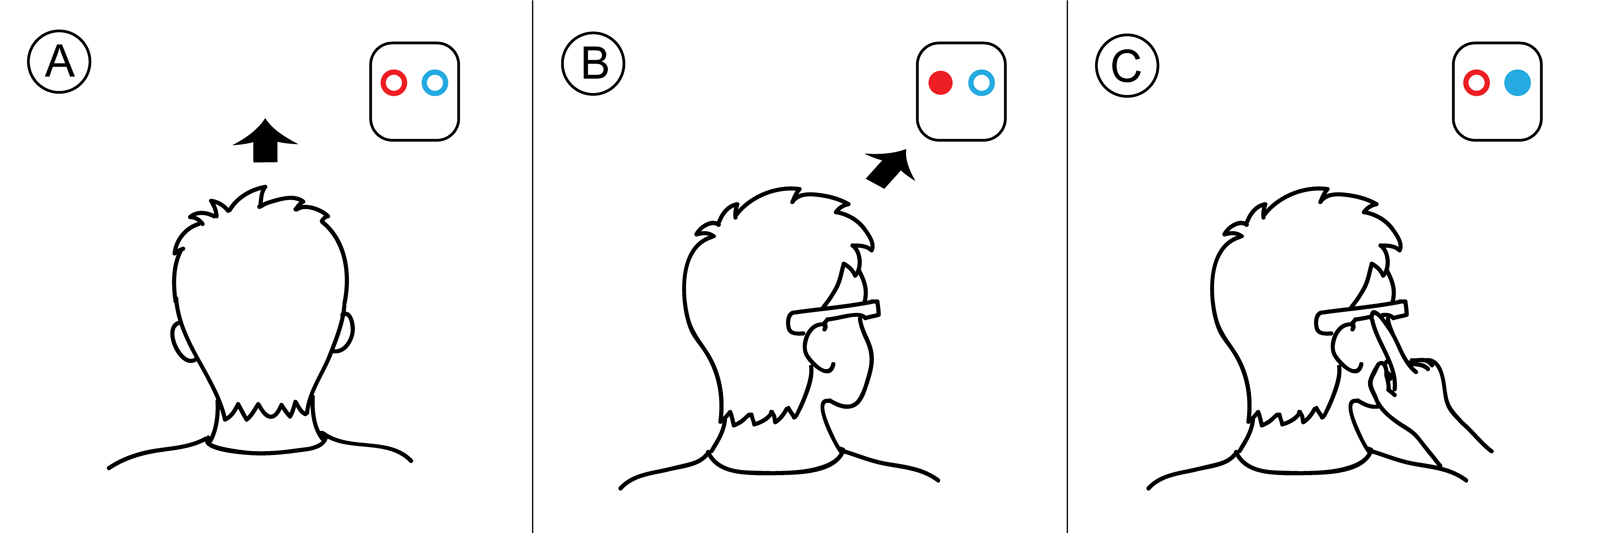
\includegraphics[width=\columnwidth]{figures/stepbystep_small.png}
\caption{Targeting interaction: when users turn towards a controllable appliance (A$\rightarrow$B), the appliance shows immediate visual feedback (red LED) (B). Users confirm that they wish to connect to this appliance with a tap (C) which triggers connection feedback (blue LED) on the appliance.}
\label{fig:interaction}
\vspace{0.1in}
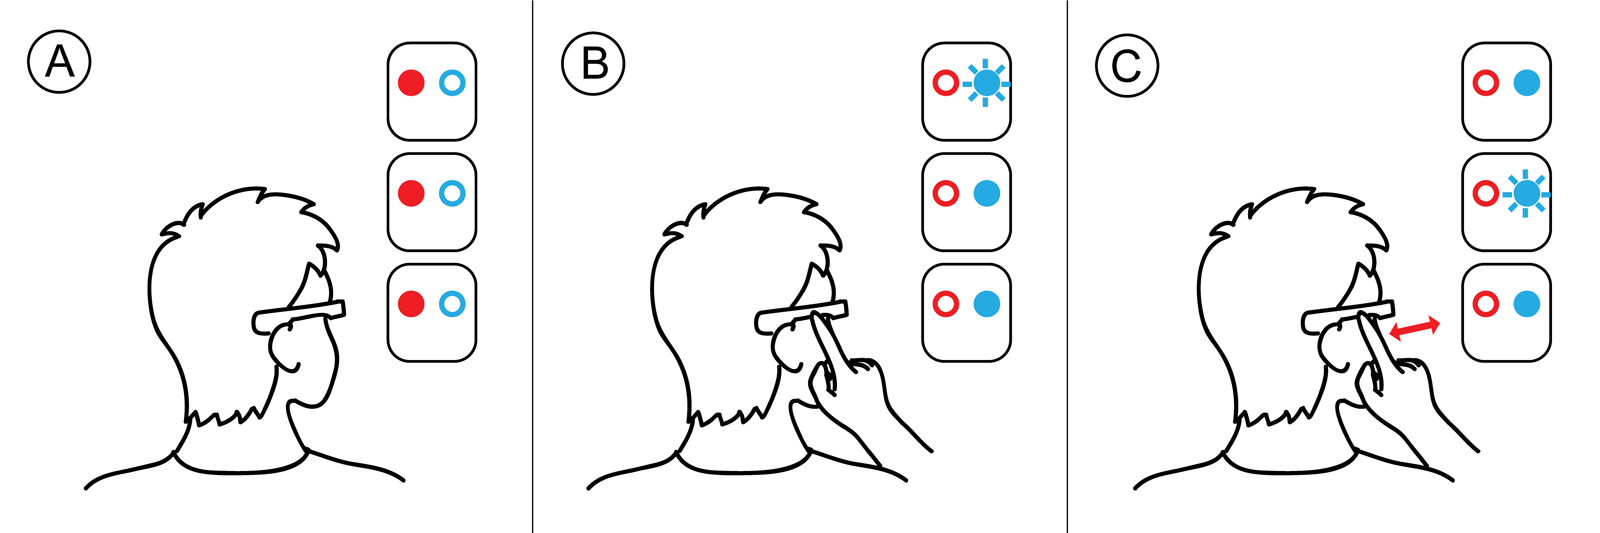
\includegraphics[width=\columnwidth]{figures/stepbystep_multi_small.png}
\caption{When multiple appliances are within range, they all have red LEDs illuminated for feedback (A). When users initiate connections, all target appliances toggle on blue LEDs while the currently selected one blinks (B). Swiping on the touchpad traverses among responding appliances (C).}
\label{fig:interaction_multi}
\end{figure}

\begin{figure}[t]
\centering
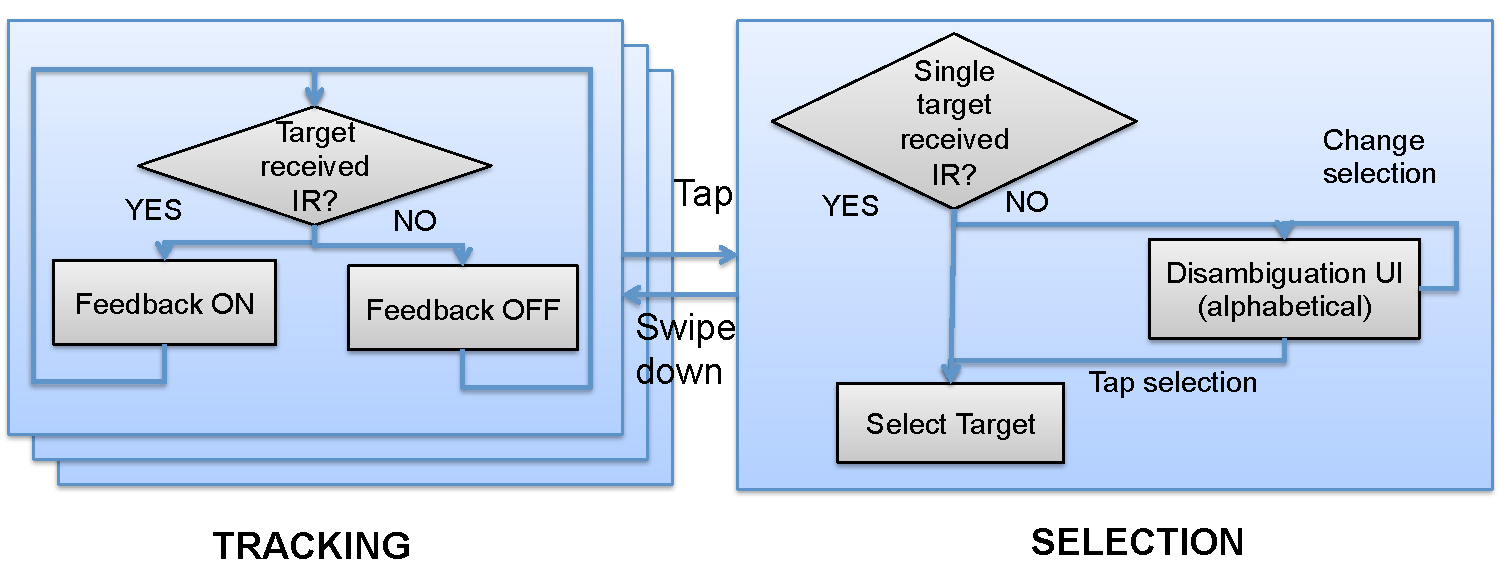
\includegraphics[width=1.0\columnwidth]{figures/selectflow01.pdf}
\caption{Head orientation selection flowchart for our first design.}
\label{fig:selectflow01}
\end{figure}

{\bf Look:} Users looking in the general direction of the intended target.
Glass periodically sends a device id through its IR emitter analogous to Patel's approach~\cite{patel_2-way_2003}. Target appliances have IR receivers and offer immediate visual feedback by toggling a red LED whenever a valid id is received (Figure~\ref{fig:interaction}B). This enables {\em scanning} the environment with one's gaze to see which appliances can be controlled.

{\bf Initiate:} Users confirm their desire to connect to an appliance by tapping on the Glass touchpad. After they are connected, the target appliance toggles on a blue LED as visual feedback (Figure~\ref{fig:interaction}C). The next section on disambiguation deals with cases in which multiple appliances received valid IR signals. At this point, all further communication switches over to the 802.15.4 wireless network so that line of sight to the target is no longer needed.

{\bf Refinement:}
Head orientation only indicates a general area of visual interest. It does not necessarily match gaze orientation as extra-ocular muscles can move the eyes. The IR beam of our device also has a certain spread . In an environment dense with potential targets, multiple targets could be within range. Users can tell when multiple feedback LEDs in the environment illuminate (Figure~\ref{fig:interaction_multi}A). To disambiguate, users can either move to adjust their head position, or, alternatively, call up a disambiguation dialog on the Glass display. The dialog presents a list filtered to only those appliances that are within IR range, while appliances also use blue LED as visual cues: all responding appliances light up LEDs while the currently selected one blinks (Figure~\ref{fig:interaction_multi}B). Users navigate the list using the touchpad (Figure~\ref{fig:interaction_multi}C), and then continue their interaction as described above.

\subsection{Implementation}
\begin{figure}[t]
\centering
\includegraphics[width=0.7\columnwidth]{figures/tube_from_top.jpg}
\caption{Our augmented Glass prototype has a frame-mounted infrared emitter.}
\label{fig:glass}
\end{figure}
\begin{figure}[t]
\centering
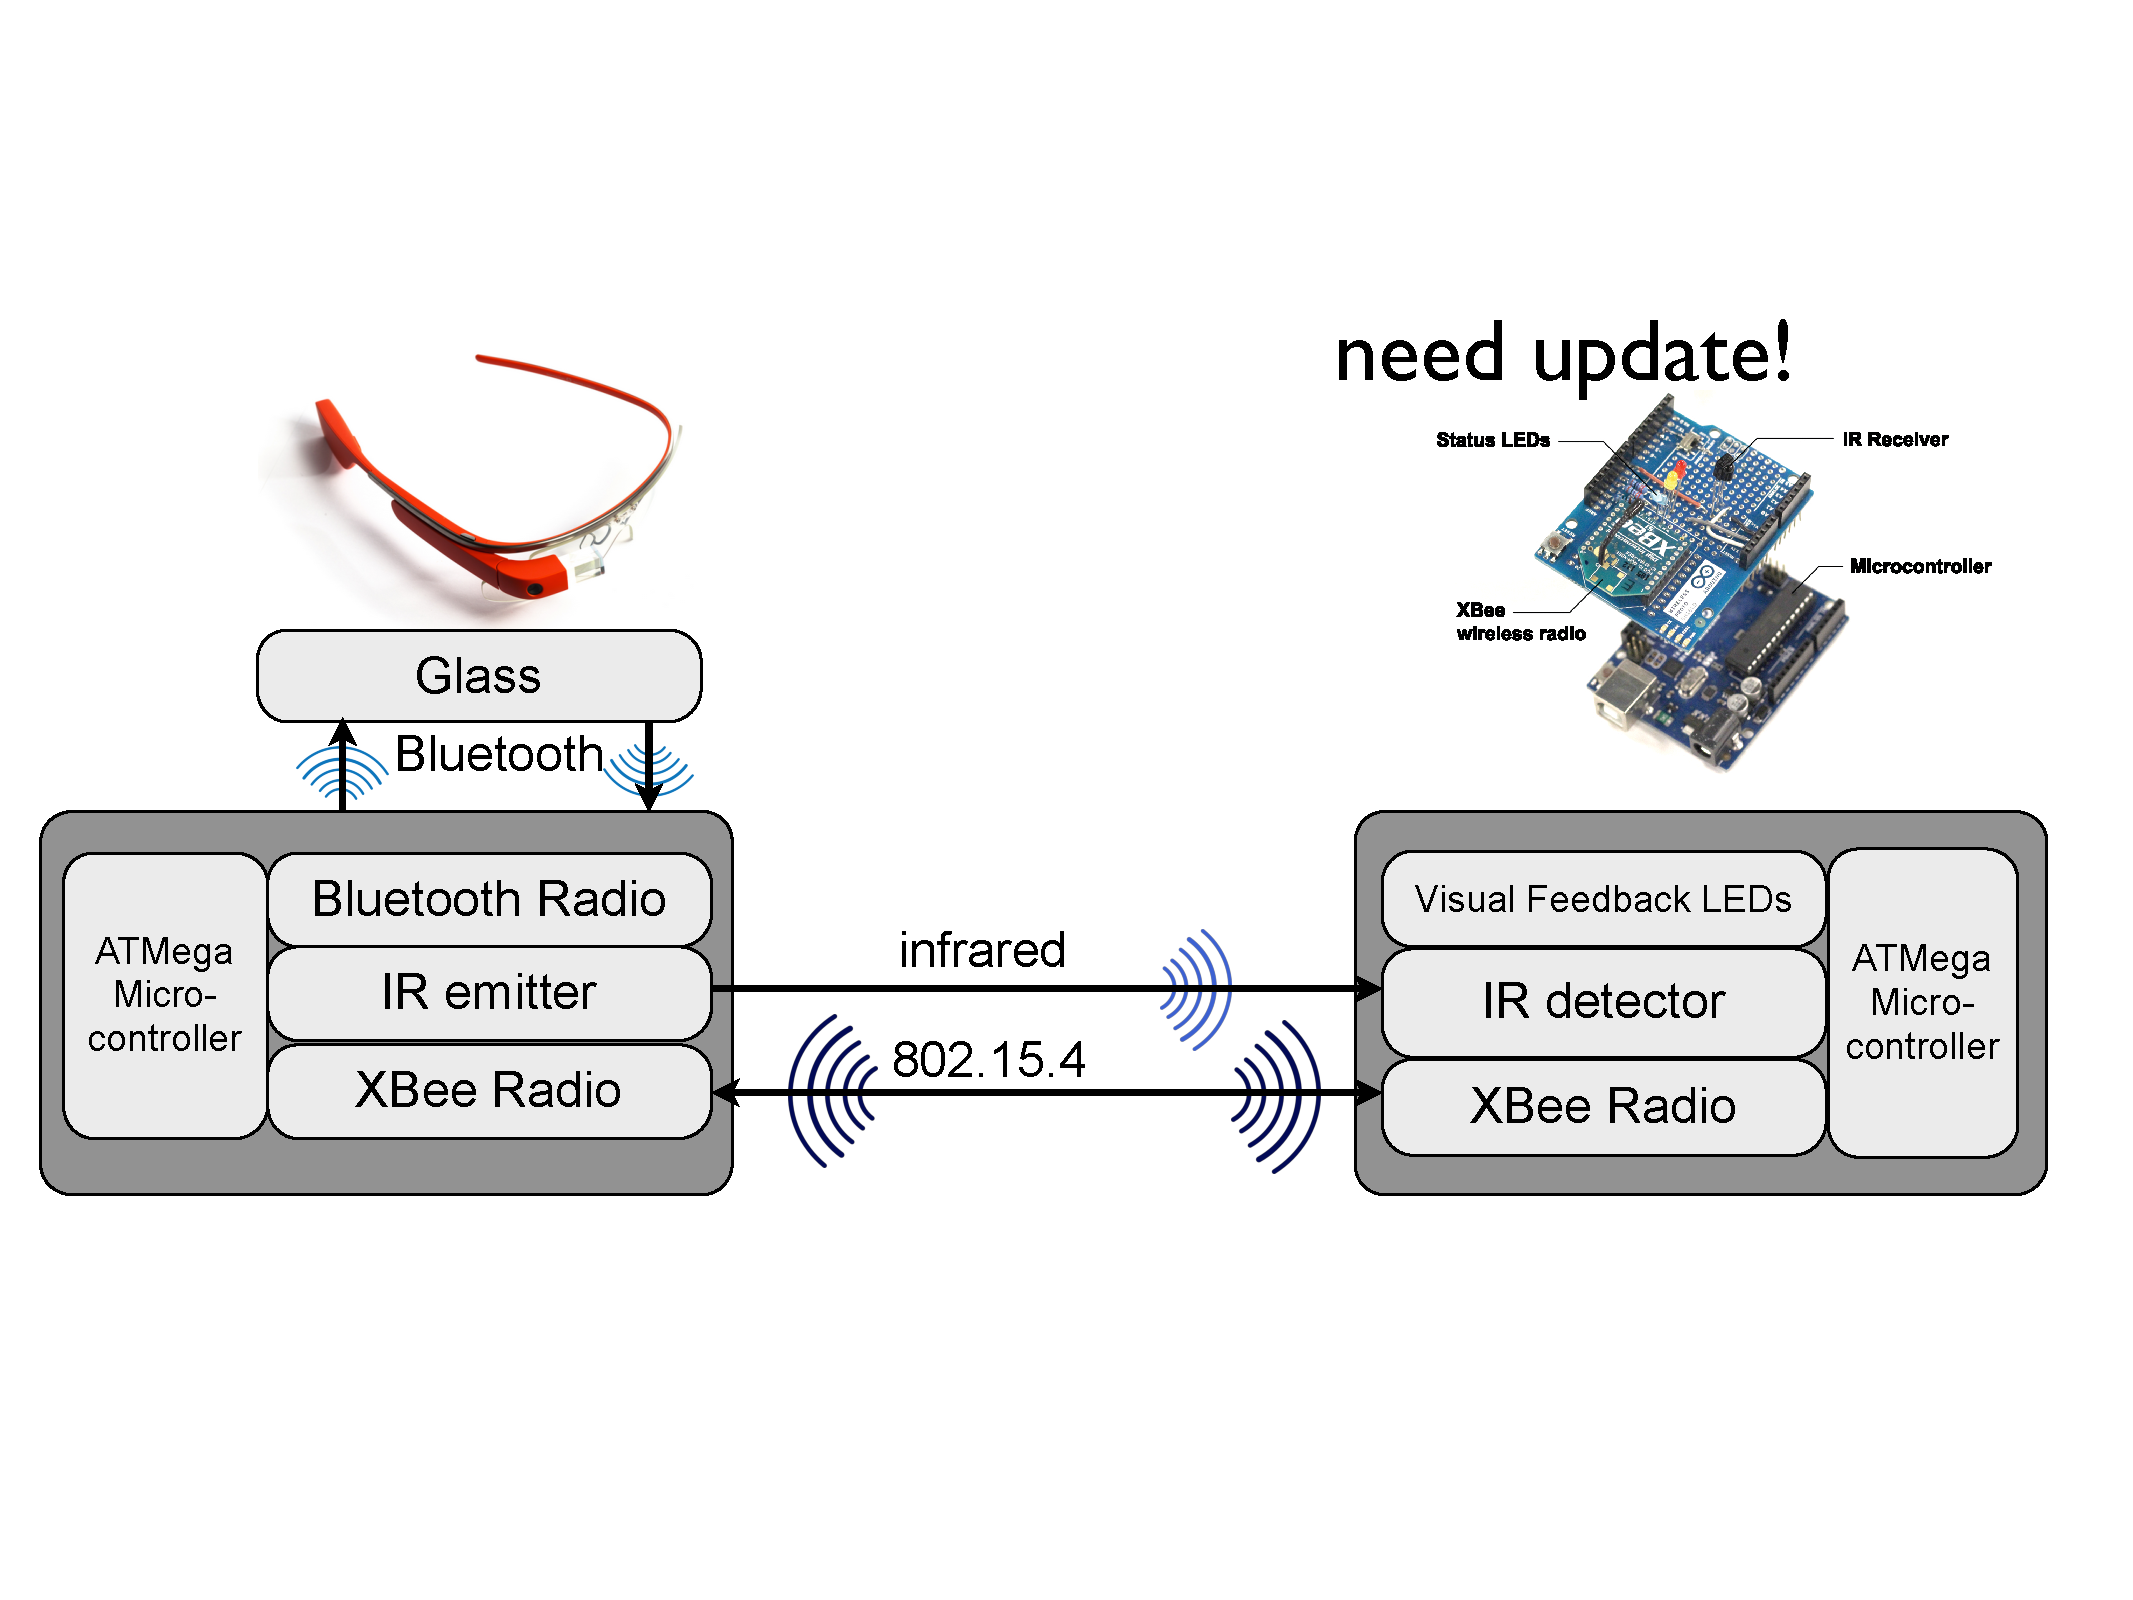
\includegraphics[width=1.0\columnwidth]{figures/architecture}
\caption{In our system architecture, selection is initiated through infrared but confirmed over 802.15.4. This permits wearers to move their head freely after connecting to an appliance. In the research prototype, users have to carry an additional microcontroller board that marshals messages between Glass' Bluetooth radio an IR/802.15.4, but our custom hardware could also be integrated into the wearable device.}
\label{fig:architecture}
\end{figure}

Our prototype consists of a Google Glass Explorer Edition device, augmented with an infrared emitter that is mounted on the frame, pointing out in the direction of the wearer's view (Figure~\ref{fig:glass}). The IR emitter LED is mounted in a \bjoern{3D printed housing which can be adjusted so the emitter can point straight forward for different head shapes}.

Our measurements suggest that IR communication can be targeted to an area about 60-120cm in diameter, up to 5m in front of the user. These values are a reasonable match for selecting targets in a room-size environment. A wider beam would lead to an increased chance of multiple appliances receiving IR signals simultaneously. A narrower beam will make targeting more challenging, given the precision constraints of human head movement.

In our prototype, Glass communicates over Bluetooth to an additional microcontroller board the user has to wear (Atmel ATMega256). This board marshals XBee to Bluetooth messages in both directions and also controls the IR LED mounted on the Glass frame (Figure~\ref{fig:architecture}). This architecture was chosen for reasons of expediency and we do not claim optimality for our design decisions. Future head-mounted devices could clearly integrate IR emitters; the choice of local wireless technology could also change. In particular, one could substitute WiFi modules or design an all-Bluetooth network.


\subsection{Device Characterization}
We determined the usable range and accuracy empirically with one IR emitter and two IR receivers. The IR emitter constantly sent out an id signal. The receivers that correctly received the signal turn their LED on for 300 ms. Our measurements suggest that IR communication can be targeted to an area about 2--4' in diameter, up to 16' in front of the user. These values are a reasonable match for selecting appliances in a room-size environment. A wider beam would lead to an increased chance of multiple appliances receiving IR signals simultaneously. A narrower beam will make targeting more challenging, given the precision constraints of human head movement.

%!TEX root = uist14.tex
\section{Study 1: Physical Target Acquisition Study}
To understand the accuracy and performance of head-orientation-based selection through our device, we carried out a comparative target acquisition study, where participants had to connect to wireless nodes distributed in a room with our technique, and with an alternate list selection approach.


\subsection{Apparatus}
In an indoor environment, 10 wireless nodes are spread across a room (Figure~\ref{fig:targeting-study-layout}). Each node is an embedded wireless system with a microcontroller, IR receiver, a wireless XBee radio, and three status LEDs %(Figure~\ref{fig:target}). %An yellow LED indicates that the device is the target that should be selected in the current trial; a red LED lights up whenever the device receives an IR signal from Glass; a blue LED shows when participants have successfully connected to a device, and is also used for disambiguation when multiple targets are within IR range. 
Next to each target, a paper sheet shows a number and letter combination, which is used for uniquely identifying the device. The numbers are the primary identifiers, ordered from left to right in the room. 

\begin{figure}[t]
\centering
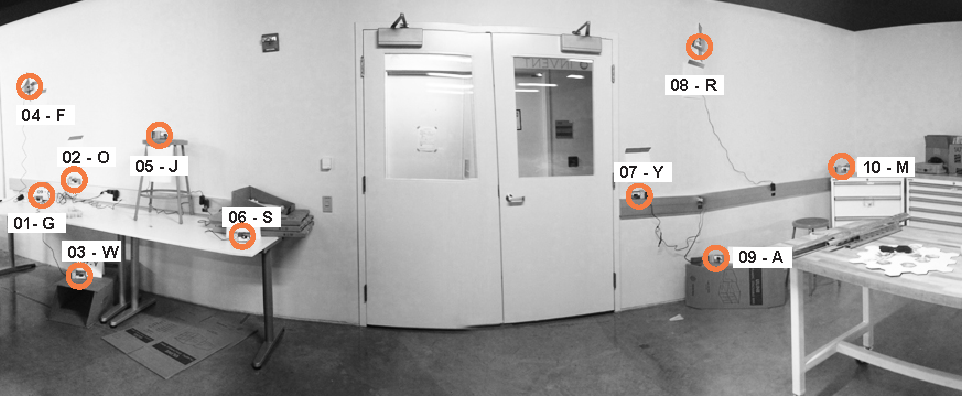
\includegraphics[width=1.0\columnwidth]{figures/targeting-study-layout.pdf}
\caption{In the targeting study, participants had to find and select one of 10 targets in a lab environment. Targets were called out by number; for the list mode condition, participants need to match numbers to letters.}
\label{fig:targeting-study-layout}
\end{figure}
%\begin{figure}[b]
%\centering
%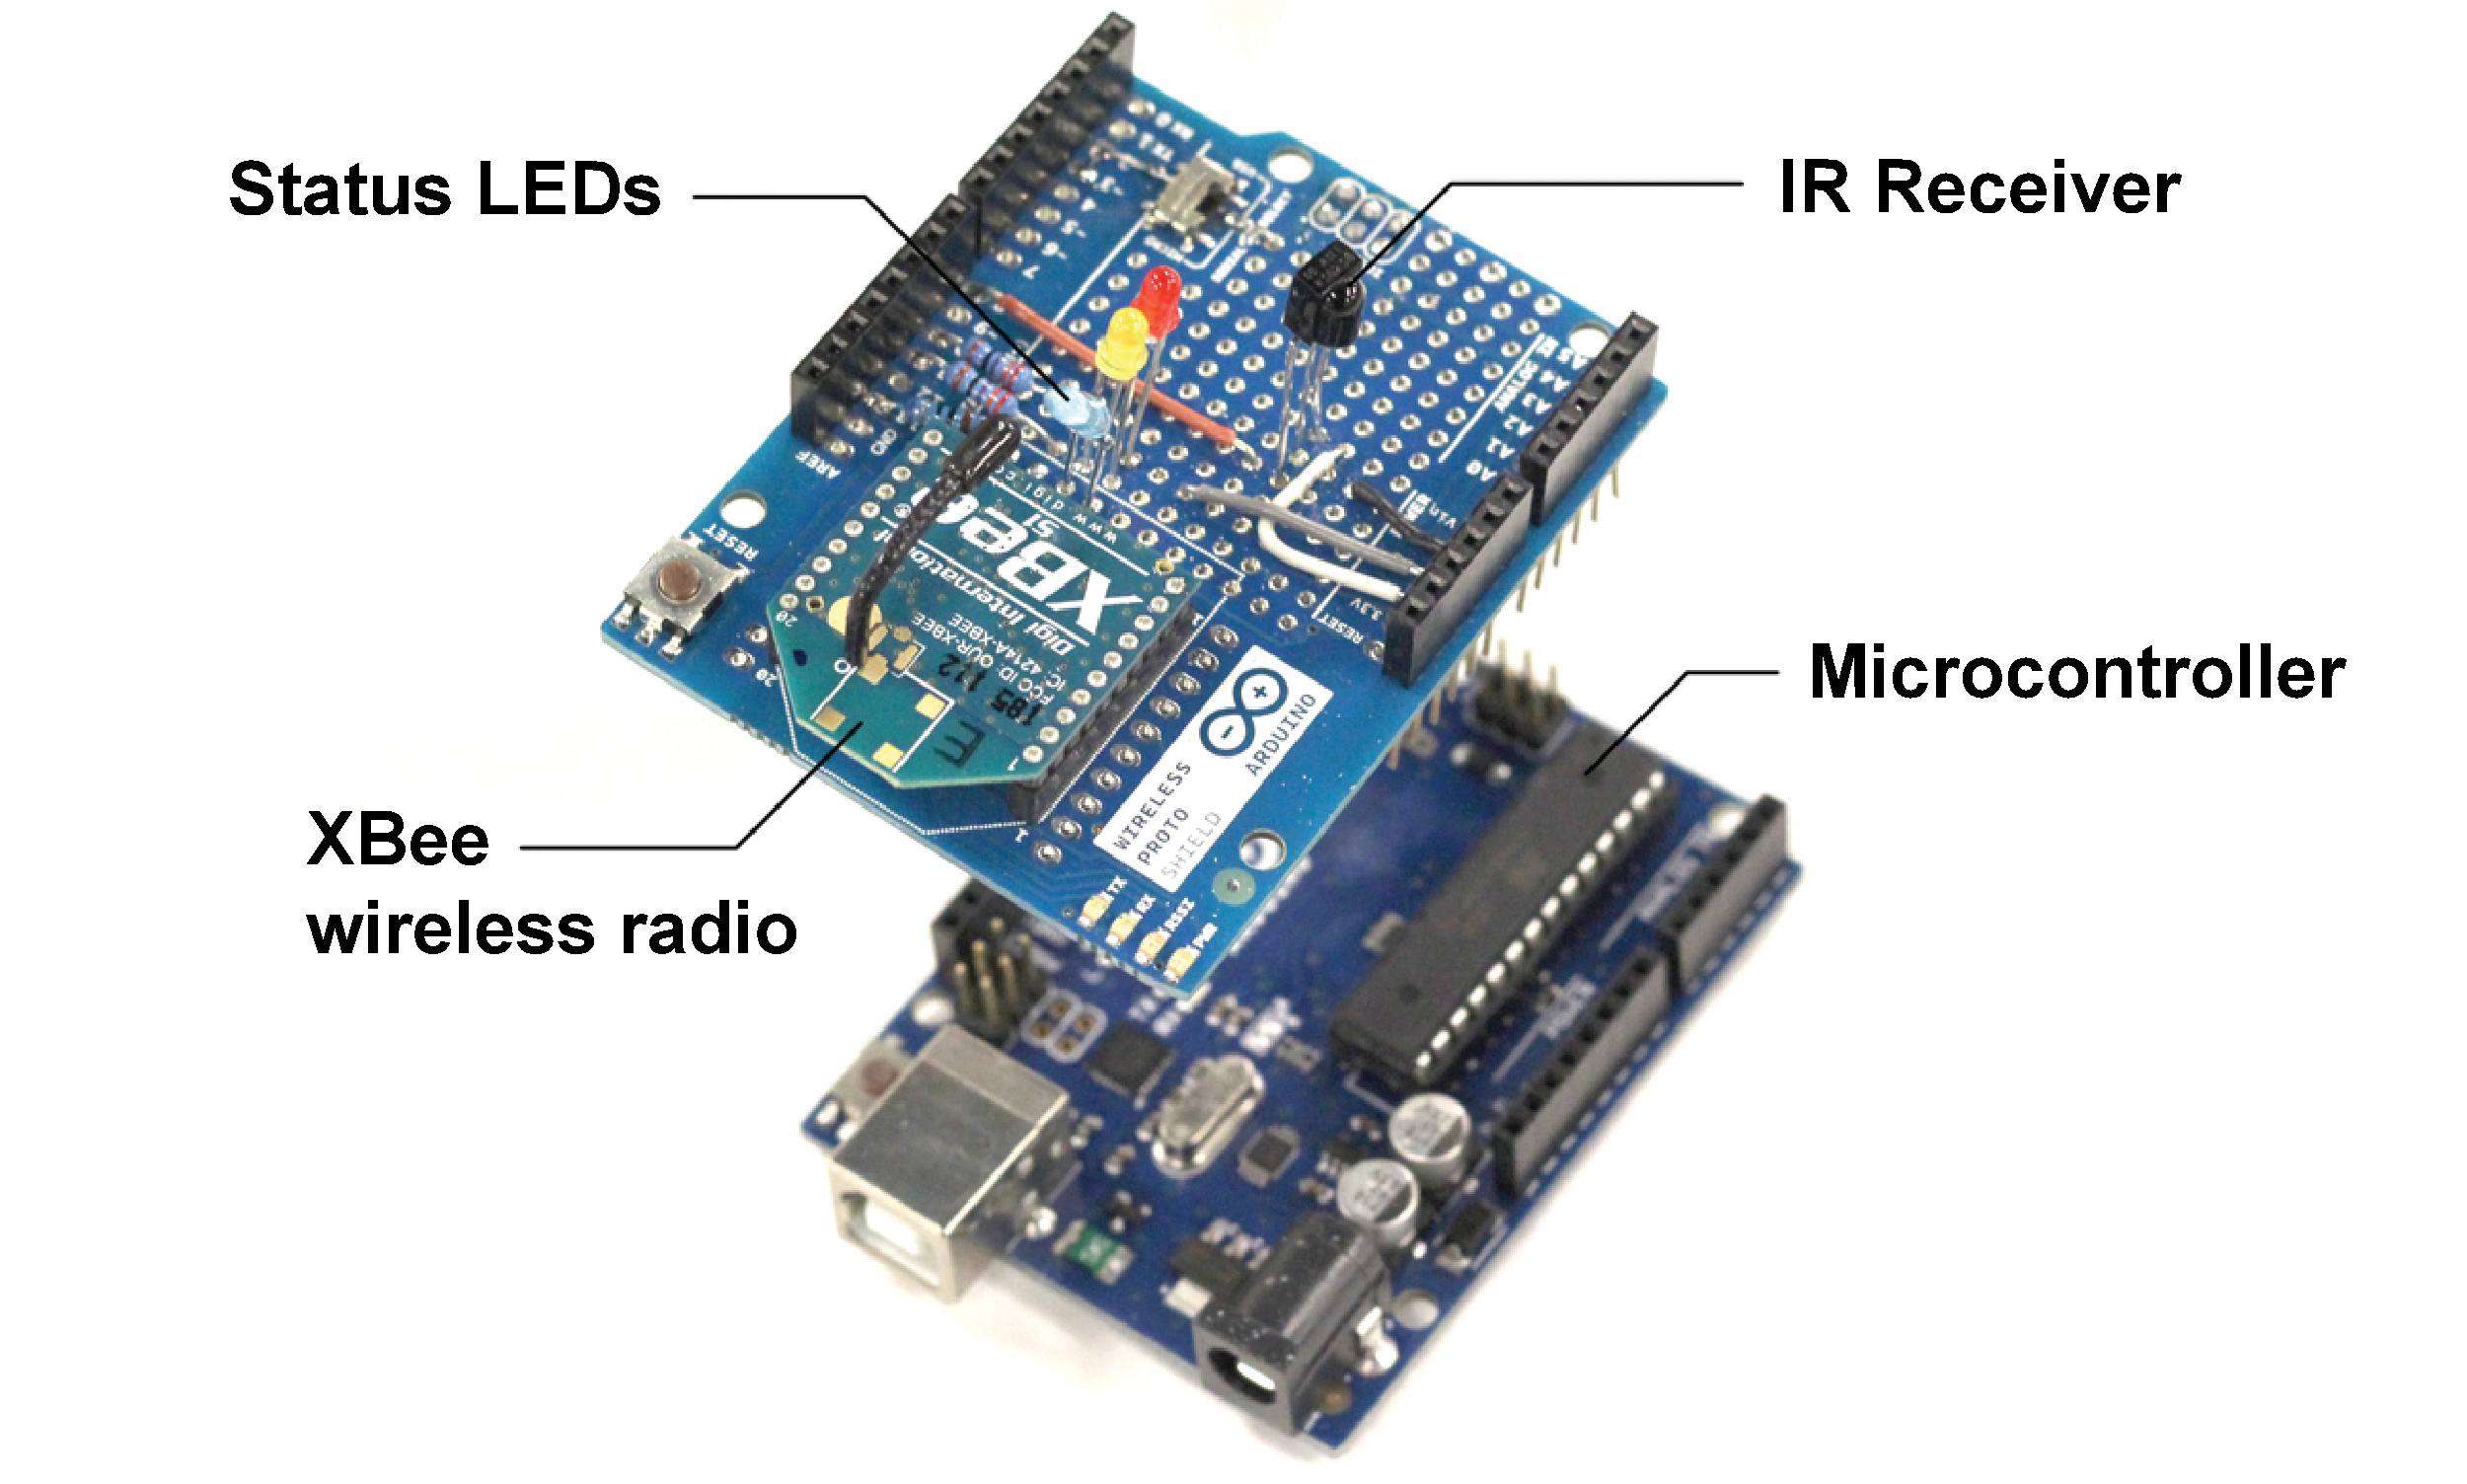
\includegraphics[width=0.8\columnwidth]{figures/study-node.pdf}
%\caption{An example node from the targeting study --- we constructed 10 such nodes - each mounted in a box.}
%\label{fig:target}
%\end{figure}

\subsection{Methodology}
In our within-subjects design, participants performed 15 target acquisition tasks each with two interaction styles. In the {\em infrared} mode condition, participants used our IR targeting approach; in the {\em list} mode condition, participants had to look up a device's letter code on the printed paper next to the device and then select that letter code from a list displayed on their Glass device. The list was navigated with swipe motions on the Glass touchpad. For each task, participants started at a fixed position in the room. The experimenter called out a number and simultaneously started a timer. Participants then had to find the corresponding device (by looking for its printed code). In the {\em infrared} mode, participants then selected and acquired the target by aiming the IR beam at the target, and confirmed their selection with a touch pad tap. If more than one target was within range, participants had to either use the disambiguation dialog or reposition themselves. In the {\em list} mode, participants had to read the letter next to the number and then select that letter by browsing a linear list shown in their Glass display. While the list was alphabetized, letter arrangement in the room was not. This design required participants to find the target in the room before starting a list navigation to keep visual search times similar in each condition.

Afterwards, participants completed a survey that elicited answers to Likert-scale questions as well as open-ended answers about their experience.

\subsection{Participants}
We recruited 14 participants from our institution. 13 had never used Glass before. 4 wore prescription glasses, which may have affected their task performance as wearing glasses beneath Glass makes it more cumbersome to secure the position of Glass and to adjust the screen to the optimal angle. Half of them performed {\em infrared} mode first and the other half did {\em list} mode first.

\subsection{Measures}
The main measures were {\bf target acquisition time}: the time required to identify, select, and connect to a wireless target device; and {\bf user preference}: which interface users preferred for the task after completing the study.

\subsection{Results}
\subsubsection{Performance data}
The time to complete each task can be broken down into the following pieces:

$t_{infrared}=t_{locate}[+t_{reorient}][+t_{disambiguate}]+t_{tap}$

$t_{list}=t_{locate}+t_{listnav}+t_{tap}$

In both conditions, participants first have to locate the target announced by the experimenter through visual search ($t_{locate}$). In the {\em infrared} mode, participants may then directly confirm their selection if only a single target was selected ($t_{tap}$). However, if they don't immediately receive feedback that their target was selected, or if multiple targets were selected, users either have change their position or head orientation ($t_{reorient}$) or they have to step through the on-screen disambiguation dialog ($t_{disambiguate}$). In the {\em list} mode, participants must scroll through the list to find the desired target identifier ($t_{listnav}$).
Thus, {\em infrared} will show a performance benefit if $(t_{reorient}+t_{disambiguate})<t_{listnav}$. This depends on the number of total devices in the environment (increasing $t_{listnav}$), and their density (which will increase $t_{disambiguate}$). 

\begin{figure}[t]
\centering
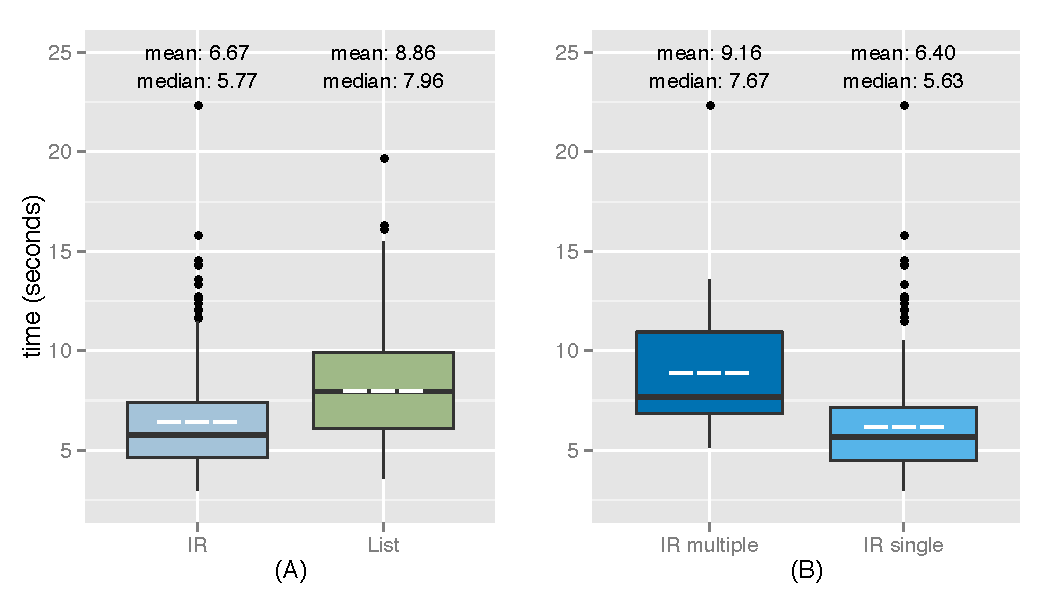
\includegraphics[width=1.0\columnwidth]{figures/R_time_by_Category.pdf}
\caption{Boxplot of task completion times for the comparison between {\em infrared} mode and {\em list} mode (A), and between IR multiple responses cases and IR single response cases (B). The centers of boxes are median values, while white dashed lines are mean values.}
\label{fig:selection-times}
\end{figure}

We first show results for 10 targets and then discuss extrapolations of these results. Average target acquisition time $t_{infrared}$ was 6.67 seconds, while $t_{list}$ was 8.86 seconds (Figure~\ref{fig:selection-times}A). This difference is significant (Student's t-test, $t(279)=-3.81, p=0.00017$). % \bjoern{you need to report the t statistic and degrees of freedom as well - t(df)= n,p=m.} 

To further understand the performance gain in {\em infrared} mode, especially the factor $t_{disambiguate}$, we compare selection times when multiple devices are targeted (and disambiguation is required) to single-device selection times (Figure~\ref{fig:selection-times}B). When there is a single device, $t_{disambiguate}$ is 0 and it takes 6.40 seconds (on average) to complete the connection. When multiple devices are in range, the time increases to 9.16 seconds, indicating 2.76 seconds required to disambiguate. Though it takes significantly longer ($t(19)=-2.7827, p=0.012$ using t-test) in the {\em multiple} case, these cases made up only 10\% of total infrared trials.
%, even we intentionally placed a few devices nearer to each other. % 19 / (19+168 )

\begin{figure}[t]
\centering
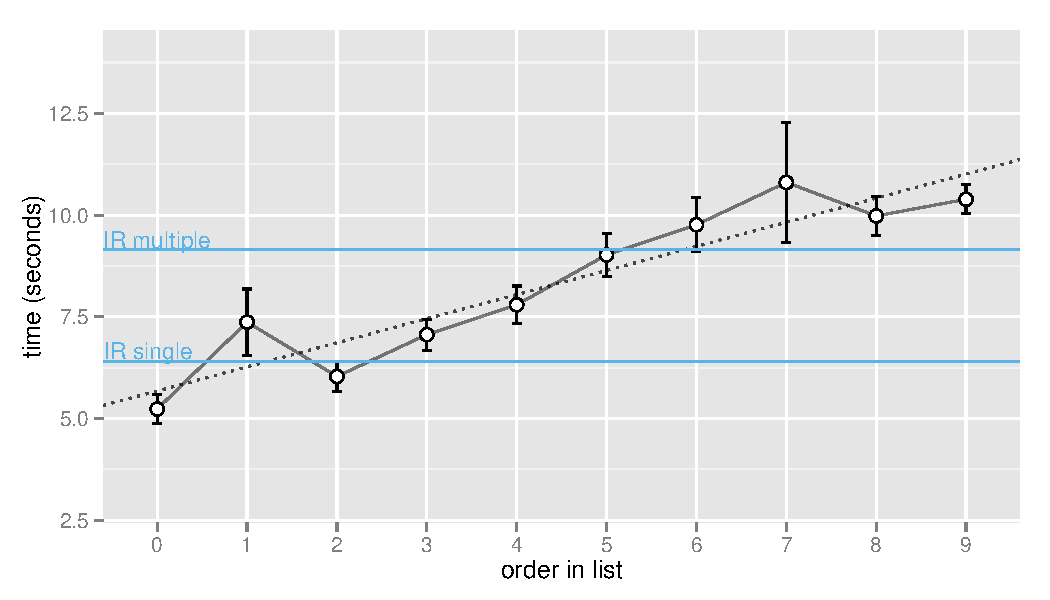
\includegraphics[width=1.0\columnwidth]{figures/R_List_by_Target.pdf}
\caption{Times taken to select a device vs.~its order in the list. The dotted line is a linear fit between the mean times and device orders. Two horizontal lines of mean target acquisition times in {\em infrared} mode are also annotated for comparison.}
 % \bjoern{Add horizontal lines at $t_{IRsingle}$ and $t_{IRmultiple}$.}
\label{fig:time-vs-list-order}
\end{figure}

For each device, $t_{listnav}$ depends on their relative position in the list. Figure~\ref{fig:time-vs-list-order} shows the time it takes to select a device (means and standard deviations) as a function of its list position - the trend line (dotted) enables extrapolation to estimate at what number of devices the {\em infrared} mode interaction techniques will outperform {\em list} mode\footnote{The higher mean value at $order=1$ is caused by one outlier when the participant tried multiple times in {\em list} mode to connect to the right target.}. From the figure, we can see that once the target's order has increased to be larger than 6, the average $t_{listnav}$ for that target would be larger than $t_{reorient} + t_{disambiguate}$. We expect that, when the number of targets keeps increasing, there would be larger time reduction in {\em infrared} mode.

% \bjoern{A linear trend is visible, and the regression returns with coefficient of determination ($R^2=0.032$). --- This R value is basically no correlation at all! try to run a correlation only on the median times. }

Participants' selection errors do occur in both conditions. However, error rates were low (1.1\% in {\em infrared} mode, and 2.9\% in {\em list} mode, respectively). This precludes us from running a more detailed analysis. 


%\subsubsection{Preference}

%Eleven of 14 users preferred infrared mode over list mode (three preferred list, one was undecided). While both interfaces were judged similarly on overall ease of connecting, list navigation was also perceived to be cumbersome. As self-report data can easily skew positive as participants try to please experimenters, we also asked participants to elucidate why they preferred one interface over the other.

%List mode had certain advantages: It was judged to be more accurate and predictable as there was always exactly one device selected in the list (\studyquote{With the list you never have to worry about accidentally picking up two targets}). Also, it did not require a clear line of sight to the target device so participants did not have to move from their starting position (\studyquote{The shortcoming of the IR mode was that you had to be a certain distance away in order for it to detect the appliance}). 

%On the other hand, list mode was judged to be more \studyquote{annoying} and tedious. The temple-based touchpad for selection was difficult to use for a participant with long hair: \studyquote{List mode was physically difficult for me to navigate, since my long hair wasn't tied back and it kept interfering with my swiping.} Another participant also commented on the ergonomic challenge of touchpad use on Glass: \studyquote{The strength of the IR mode was that I didn't have to use my fingers as much to control. If the items were spaced relatively far apart, it was easy to select a specific appliance.}

%One noted benefit of infrared mode was a feeling that it was \studyquote{more direct [than list mode]}, allowing users to focus on the targeted objects instead of the screen. One subject called it \studyquote{natural to interact with things just by looking at them}. Another mentioned that \studyquote{it's really convenient that what I'm looking at is what I'm targeting}. 

%A few perceived weaknesses of infrared mode were the necessity to move the head in order to control a device and the imperfect mapping of gaze to target. One participant said that it was \studyquote{awkward to be aiming your head at things, tweaking back and forth to get it right}. Another noted that observing the head movement didn't capture the site of her attention, because \studyquote {eye movement is an important part of how people look around}. Users had to learn the usable angle of the IR emitter before they became successful at controlling the devices: \studyquote{I had to compensate by tilting my head up a little bit.}
%!TEX root = uist14.tex
\section{Iteration 2: IR Intensity refinement}

\bjoern{The results of the first study show that head orientation targeting can outperform linear list selection, but that disambiguation (or refinement step, need to decide on consistent terminology) is costly.

Our approach to avoid paying this penalty is to provide more information to the system which target is more likely than another to be the intended selection. We do so by collecting received IR signal strength at each target node and comparing measurements of all candidate targets.}

\subsection{Interaction Flow}
\bjoern{
Intensity data is used in two ways (see Figure~\ref{fig:selectflow02}): 1) the difference in intensity between the strongest and second target exceeds a threshold, the target with the strongest received signal is automatically selected; 2) if the difference falls below the threshold, the refinement UI from the previous iteration is displayed, but items are ordered in decreasing intensity. This should maximize the chance of being able to confirm the intended target without additional UI navigation actions}.


\begin{figure}[t]
\centering
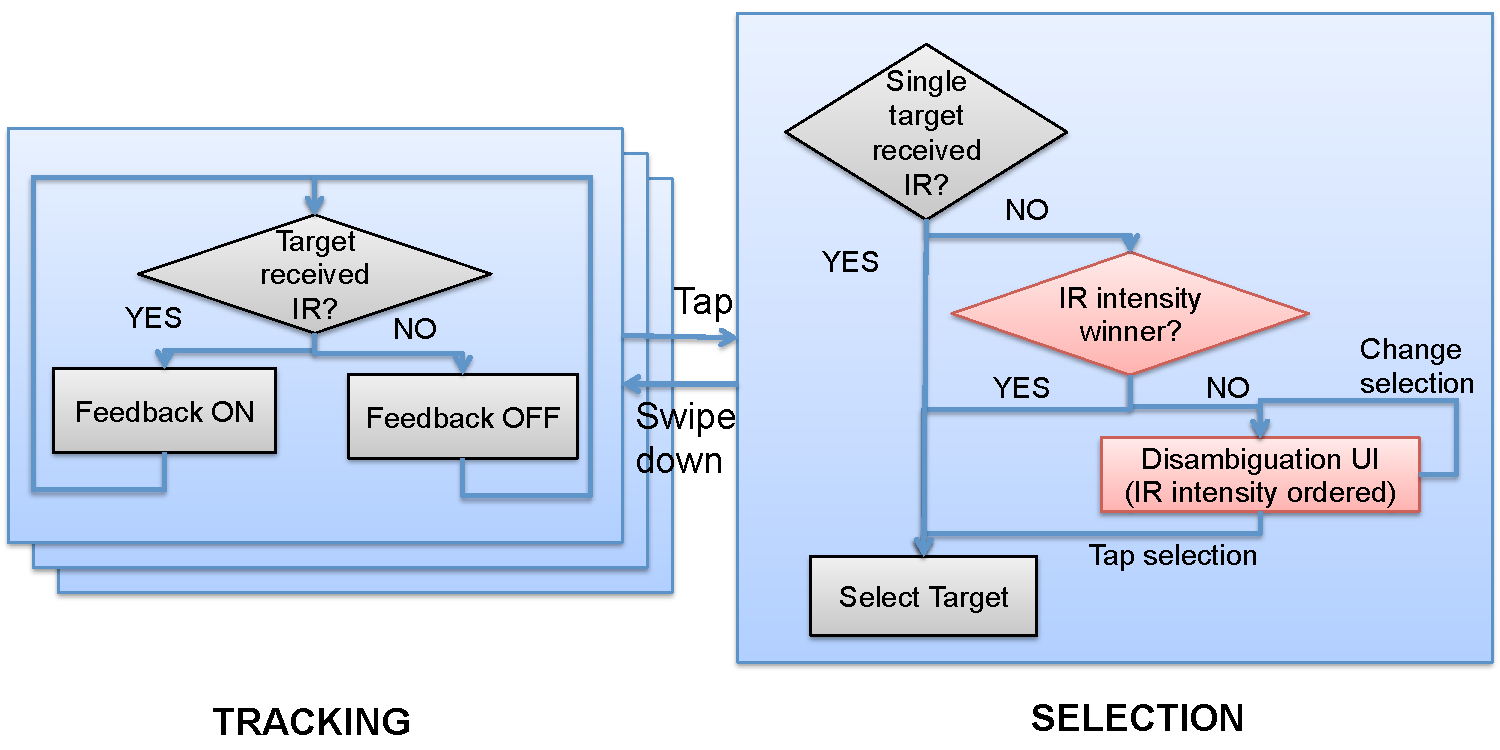
\includegraphics[width=1.0\columnwidth]{figures/selectflow02.pdf}
\caption{Head orientation selection flowchart for our second design with IR intensity measurement.}
\label{fig:selectflow02}
\end{figure}

\subsection{Implementation}
\bjoern{we use sensor X and LED y which give useful readings at up to N feet. Intensity falls of as $1/d^2$ with distance and approximately $xyz$ with angle. We empirically set the threshold for automatic selection without refinement at Z.}\bjoern{maybe show some measurements for intensity based on distance and angle as we had discussed a while ago. not essential. }

%!TEX root = uist14.tex
\section{Study2: Benefits of IR Intensity refinement}
\bjoern{write this with analogous structure as study 1 and focus on the comparisons we discussed:
1) Chi-square test of required refinement dialogs; 2) chi-square of number of times the first item in the UI was appropriate; 3) t-test of selection times; 4) comparison of error rates (likely, IR will be higher - that's the price to pay for a smarter technique).}

%!TEX root = uist14.tex
\section{Iteration 3: Orientation-based refinement}
\bjoern{While taking IR intensity into account further reduced the need for manual refinement and increased performance, the UI navigation scheme is problematic - it is not spatially related in any meaningful way to the layout of targets in a room. A better interaction technique would respect that ordering. For example, when refinement is needed, tilting the head slightly to the right could select the target that's adjacent to the right of the currently selected target.

Such spatial navigation requires knowledge about the layout of targets in the environment. However, one of the strengths of our technique so far is that it does not require any map ahead of time. To enable some spatial navigation, we introduce a final iteration in which we build up a spatial data structure by demonstration (i.e., the user looks around the room) and then leverage that data structure during the refinement step of our interaction.}

\bjoern{This technique is based on the assumption that users will generally select targets in indoor environments where targets are spread around the periphery. These assumptions enable us to use orientation data without knowing the user's absolute position.}

\subsection{Implementation}
\bjoern{give implementation details}

\subsection{Informal User Feedback}
\bjoern{We informally evaluate this technique with N users: ...}
%\section{Disambiguation Techniques}
\label{sec:disamb-techn}

This section discusses the three different disambiguation techniques we have proposed.

\subsection{Using IR Intensity}
\label{sec:using-ir-intensity}

\subsection{Using Glass Sensors}
\label{sec:using-glass-sensors}

\subsection{Manual Disambiguation}
\label{sec:manu-disamb}



%%% Local Variables: 
%%% mode: latex
%%% TeX-master: "uist14"
%%% End: 

%
\section{Evaluation}
\label{sec:evaluation}

This section we present our work on the evaluation and user study.


%%% Local Variables: 
%%% mode: latex
%%% TeX-master: "uist14"
%%% End: 

\section{Applications}
\label{sec:applications}

In this section we describe four possible applications that can be built on top of the head orientation-based selection. We focus our discussion on the ``universal remote control'' system. 

%%% Local Variables: 
%%% mode: latex
%%% TeX-master: "uist14"
%%% End: 


\section{Discussion}
\label{sec:discussion}

We discuss a few issues with the system.
%%% Local Variables: 
%%% mode: latex
%%% TeX-master: "uist14"
%%% End: 

\section{Conclusion}
We introduced a novel method for selecting and controlling smart appliances in physical spaces through  infrared targeting based on head orientation. The design takes advantage of the fact that visual attention can express intention, makes it ituitive and helps users remain their focus in the physical world. It addresses the naming and scaling challenges faced by handheld mobile devices. While we present a prototype approach that requires that the user carry additional hardware, all parts can readily be miniaturized and integrated into future head-worn hardware. We also introduced a disambiguation technique in case head orientation is not sufficient to determine a unique target. We characterized our devices performance, arguing that it is matched well to the amount of head movement people can control without strain. A target acquisition study showed that the technique is efficient; a home control scenario showed promise but also limitations when trying to control complex appliances. As our environment continues to be populated by a swarm of sensing and actuation devices, methods to interrogate and control our smart environments may become increasingly important.
%\section{Acknowledgments}
%We thank our user study participants and the a

\iftoggle{anonymous}{
% no acks in anonymous submission
}{
  \section{Acknowledgments}
  
  This work was supported in part by the TerraSwarm Research Center, one of six centers supported by the STARnet phase of the Focus Center Research Program (FCRP) a Semiconductor Research Corporation program sponsored by MARCO and DARPA. Additional support was provided by a Sloan Foundation Fellowship and a Google Research Award.
}
%figure template:
%\begin{figure}[!h]
%\centering
%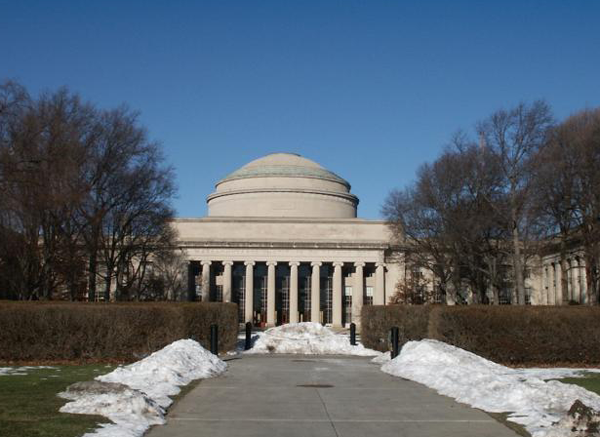
\includegraphics[width=1.0\columnwidth]{Figure1}
%\caption{With Caption Below, be sure to have a good resolution image
%  (see item D within the preparation instructions).}
%\label{fig:figure1}
%\end{figure}

% Balancing columns in a ref list is a bit of a pain because you
% either use a hack like flushend or balance, or manually insert
% a column break.  http://www.tex.ac.uk/cgi-bin/texfaq2html?label=balance
% multicols doesn't work because we're already in two-column mode,
% and flushend isn't awesome, so I choose balance.  See this
% for more info: http://cs.brown.edu/system/software/latex/doc/balance.pdf
%
% Note that in a perfect world balance wants to be in the first
% column of the last page.
%
% If balance doesn't work for you, you can remove that and
% hard-code a column break into the bbl file right before you
% submit:
%
% http://stackoverflow.com/questions/2149854/how-to-manually-equalize-columns-
% in-an-ieee-paper-if-using-bibtex
%
% Or, just remove \balance and give up on balancing the last page.
%
%% \balance

\bibliographystyle{acm-sigchi}
\bibliography{uist14}
\end{document}
